\subsection{W+Jets MC Modelling Validation from CR1}
\label{sec:cr1}


The estimate of the uncertainty on this background is based on CR1, 
defined by applying the full signal selection, including the isolated track veto, but requiring 0 b-tags
(CSV medium working point as described in Sec.~\ref{sec:selection}). 
The sample is dominanted by \wjets\ and is thus used to validate the MC modelling of this background. 

In Table~\ref{tab:cr1mtsf} we show the amount that we need to scale the Wjets MC
by in order to have agreement between data and Monte Carlo in the $M_T$ peak 
region, defined as $60 < M_T < 100$ GeV.  These scale factors are not terribly 
important, but it is reassuring that they are not too different from
1.  [UPDATE WITH TRIGGER EFFICIENCIES]


\begin{table}[!h]
\begin{center}
\begin{tabular}{l||c||c|c|c|c|c}
\hline
Sample              & CR1PRESEL & CR1A & CR1B & CR1C & CR1D & CR1E\\
\hline
\hline
Muon \mt-SF 	  & $0.92 \pm 0.02$ & $0.97 \pm 0.03$ & $0.90 \pm 0.04$ & $0.91 \pm 0.06$ & $0.93 \pm 0.09$ & $0.98 \pm 0.13$ \\
\hline
\hline
Electron \mt-SF 	  & $0.94 \pm 0.02$ & $0.90 \pm 0.04$ & $0.84 \pm 0.05$ & $0.80 \pm 0.07$ & $0.83 \pm 0.10$ & $0.77 \pm 0.13$ \\
\hline
\end{tabular}
\caption{ \mt\ peak Data/MC scale factors applied to the single lepton
  samples and \ttdl. The raw MC is used for backgrounds from rare
  processes. CR1PRESEL refers to a sample with $\met>50$ GeV.
  The uncertainties are statistical only.
\label{tab:cr1mtsf}}
\end{center}
\end{table}


In Table~\ref{tab:cr1yields} we compare the data and MC yields in the four $M_T$ signal regions
and in a looser control region.  We also derive the data/MC scale factors 
$SFR^{e}_{wjet}$ and  $SFR^{\mu}_{wjet}$.  The underlying \met\ and $M_T$ distributions
are shown in Fig.~\ref{fig:cr1met}  and~\ref{fig:cr1mtrest}

\begin{table}[!h]
\begin{center}
{\footnotesize
\begin{tabular}{l||c||c|c|c|c|c}
\hline
Sample              & CR1PRESEL & CR1A & CR1B & CR1C & CR1D & CR1E\\
\hline
\hline
Muon MC 		  & $480 \pm 22$ & $173 \pm 5$ & $114 \pm 4$ & $40 \pm 2$ & $16 \pm 1$ & $8 \pm 1$ \\
Muon Data 		  & $629$ & $238$ & $139$ & $45$ & $12$ & $8$ \\
\hline
Muon Data/MC SF: ($SFR^{\mu}_{wjet}$) 	  & $1.31 \pm 0.08$ & $1.37 \pm 0.10$ & $1.22 \pm 0.11$ & $1.12 \pm 0.18$ & $0.75 \pm 0.23$ & $0.99 \pm 0.37$ \\
\hline
\hline
Electron MC 		  & $330 \pm 8$ & $118 \pm 4$ & $79 \pm 3$ & $29 \pm 2$ & $13 \pm 1$ & $5 \pm 1$ \\
Electron Data 		  & $473$ & $174$ & $100$ & $36$ & $16$ & $5$ \\
\hline
Electron Data/MC SF: ($SFR^e_{wjet}$) 	  & $1.43 \pm 0.07$ & $1.47 \pm 0.12$ & $1.27 \pm 0.14$ & $1.23 \pm 0.22$ & $1.26 \pm 0.34$ & $1.07 \pm 0.51$ \\
\hline
\end{tabular}}
\caption{ Yields in \mt\ tail comparing the MC prediction (after
  applying SFs) to data. CR1PRESEL refers to a sample with $\met>50$
  GeV and $\mt>150$ GeV.
  The uncertainties are statistical only. 
\label{tab:cr1yields}}
\end{center}
\end{table}


\begin{table}[!h]
\begin{center}
{\footnotesize
\begin{tabular}{l||c||c|c|c|c|c}
\hline
Sample              & CR1PRESEL & CR1A & CR1B & CR1C & CR1D & CR1E\\
\hline
\hline
Muon W+jets MC 		  & $300 \pm 23$ & $84 \pm 5$ & $52 \pm 4$ & $20 \pm 2$ & $9 \pm 2$ & $5 \pm 1$ \\
Muon Data - non-W+jets MC 		  & $449 \pm 26$ & $149 \pm 16$ & $78 \pm 12$ & $25 \pm 7$ & $5 \pm 4$ & $5 \pm 3$ \\
\hline
Muon Data/MC SF: ($SFR^{\mu}_{wjet}$) 	  & $1.50 \pm 0.14$ & $1.77 \pm 0.21$ & $1.49 \pm 0.26$ & $1.25 \pm 0.38$ & $0.56 \pm 0.39$ & $0.98 \pm 0.62$ \\
\hline
\hline
Electron W+jets MC 		  & $192 \pm 8$ & $55 \pm 4$ & $36 \pm 3$ & $14 \pm 2$ & $6 \pm 1$ & $3 \pm 1$ \\
Electron Data - non-W+jets MC 		  & $335 \pm 22$ & $111 \pm 13$ & $58 \pm 10$ & $20 \pm 6$ & $10 \pm 4$ & $3 \pm 2$ \\
\hline
Electron Data/MC SF: ($SFR^e_{wjet}$) 	  & $1.74 \pm 0.14$ & $2.02 \pm 0.29$ & $1.58 \pm 0.32$ & $1.49 \pm 0.50$ & $1.50 \pm 0.70$ & $1.10 \pm 0.80$ \\
\hline
\end{tabular}}
\caption{ Yields in \mt\ tail comparing the \wjets\ MC prediction (after
  applying SFs) to data after subtracting the non-\wjets\ component. CR1PRESEL refers to a sample with $\met>50$
  GeV and $\mt>150$ GeV.
  The uncertainties are statistical only. 
\label{tab:cr1wyields}}
\end{center}
\end{table}


\begin{figure}[hbt]
  \begin{center}
        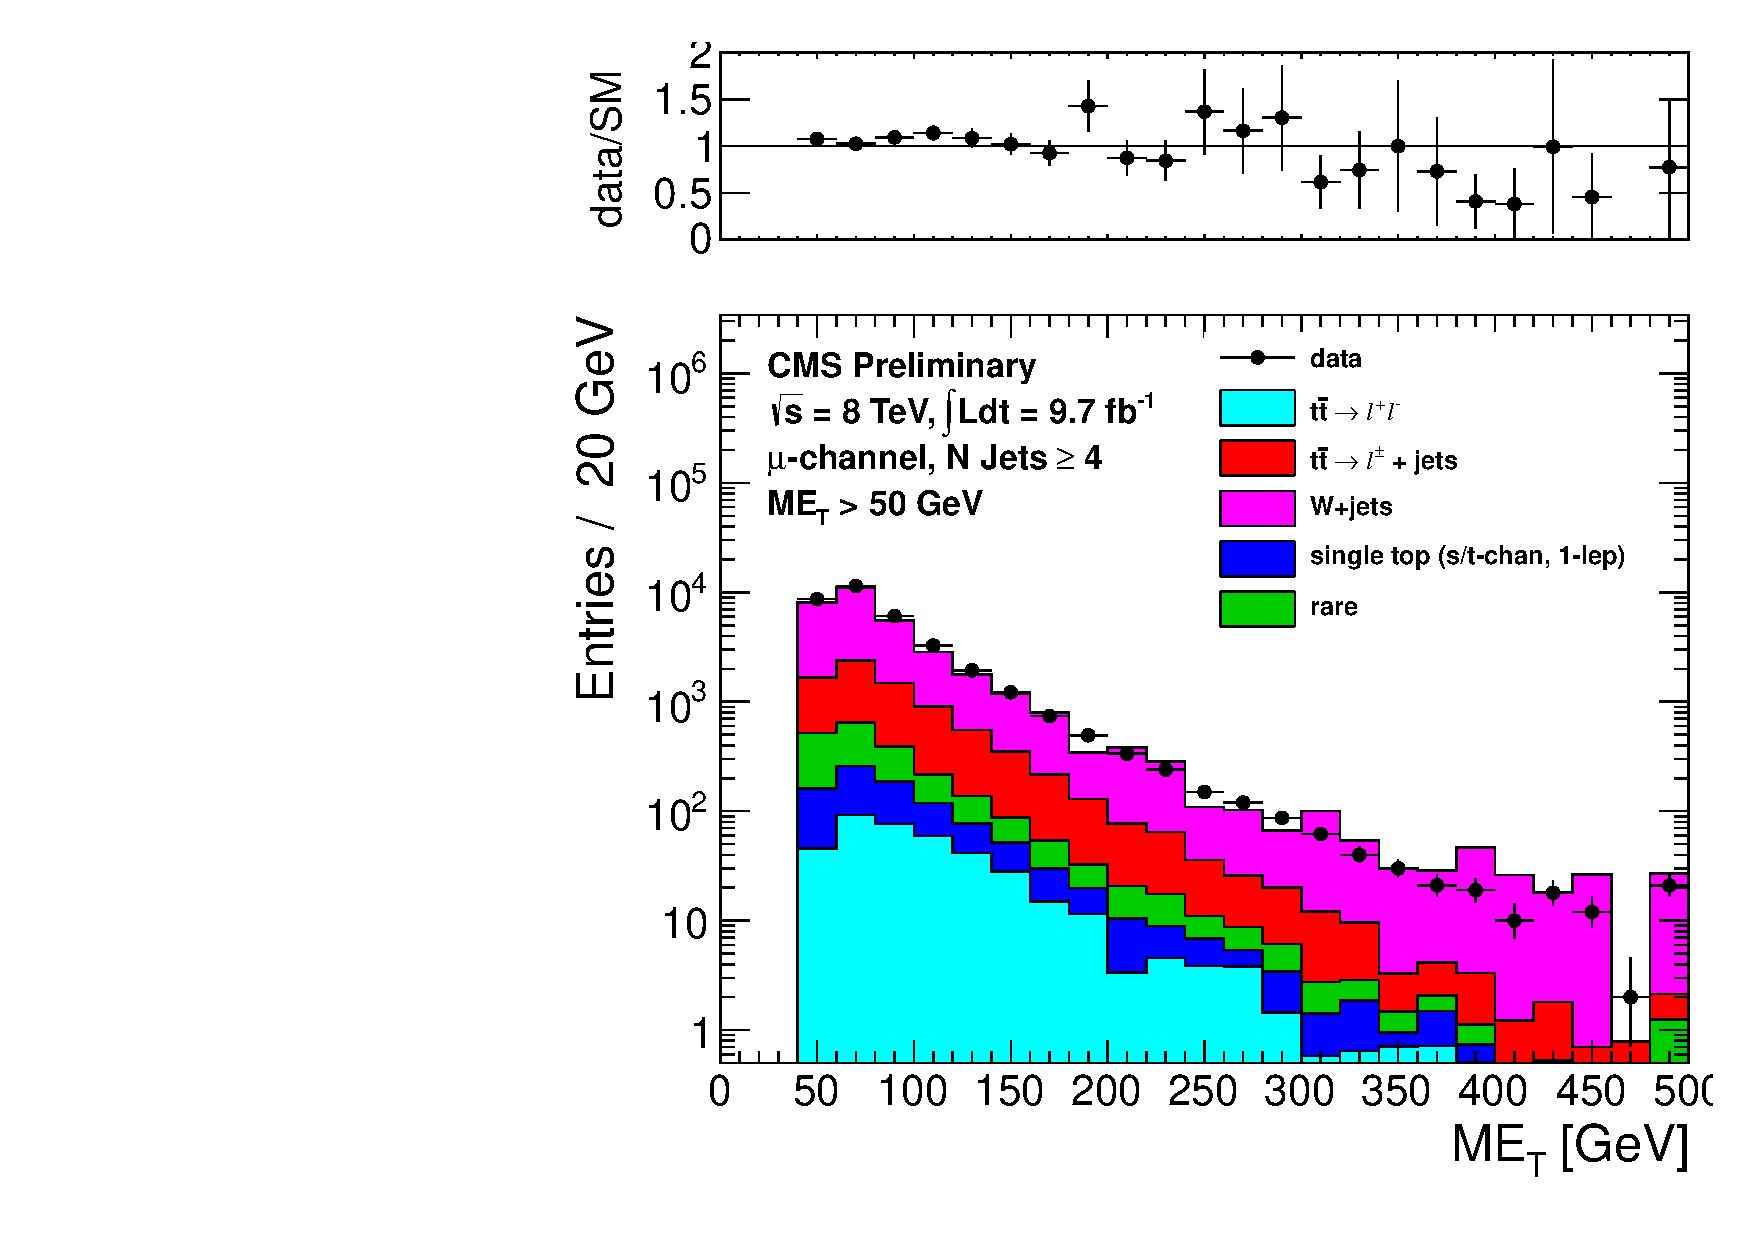
\includegraphics[width=0.5\linewidth]{plots/CR1plots/met_met50_leadmuo_nj4.pdf}%
        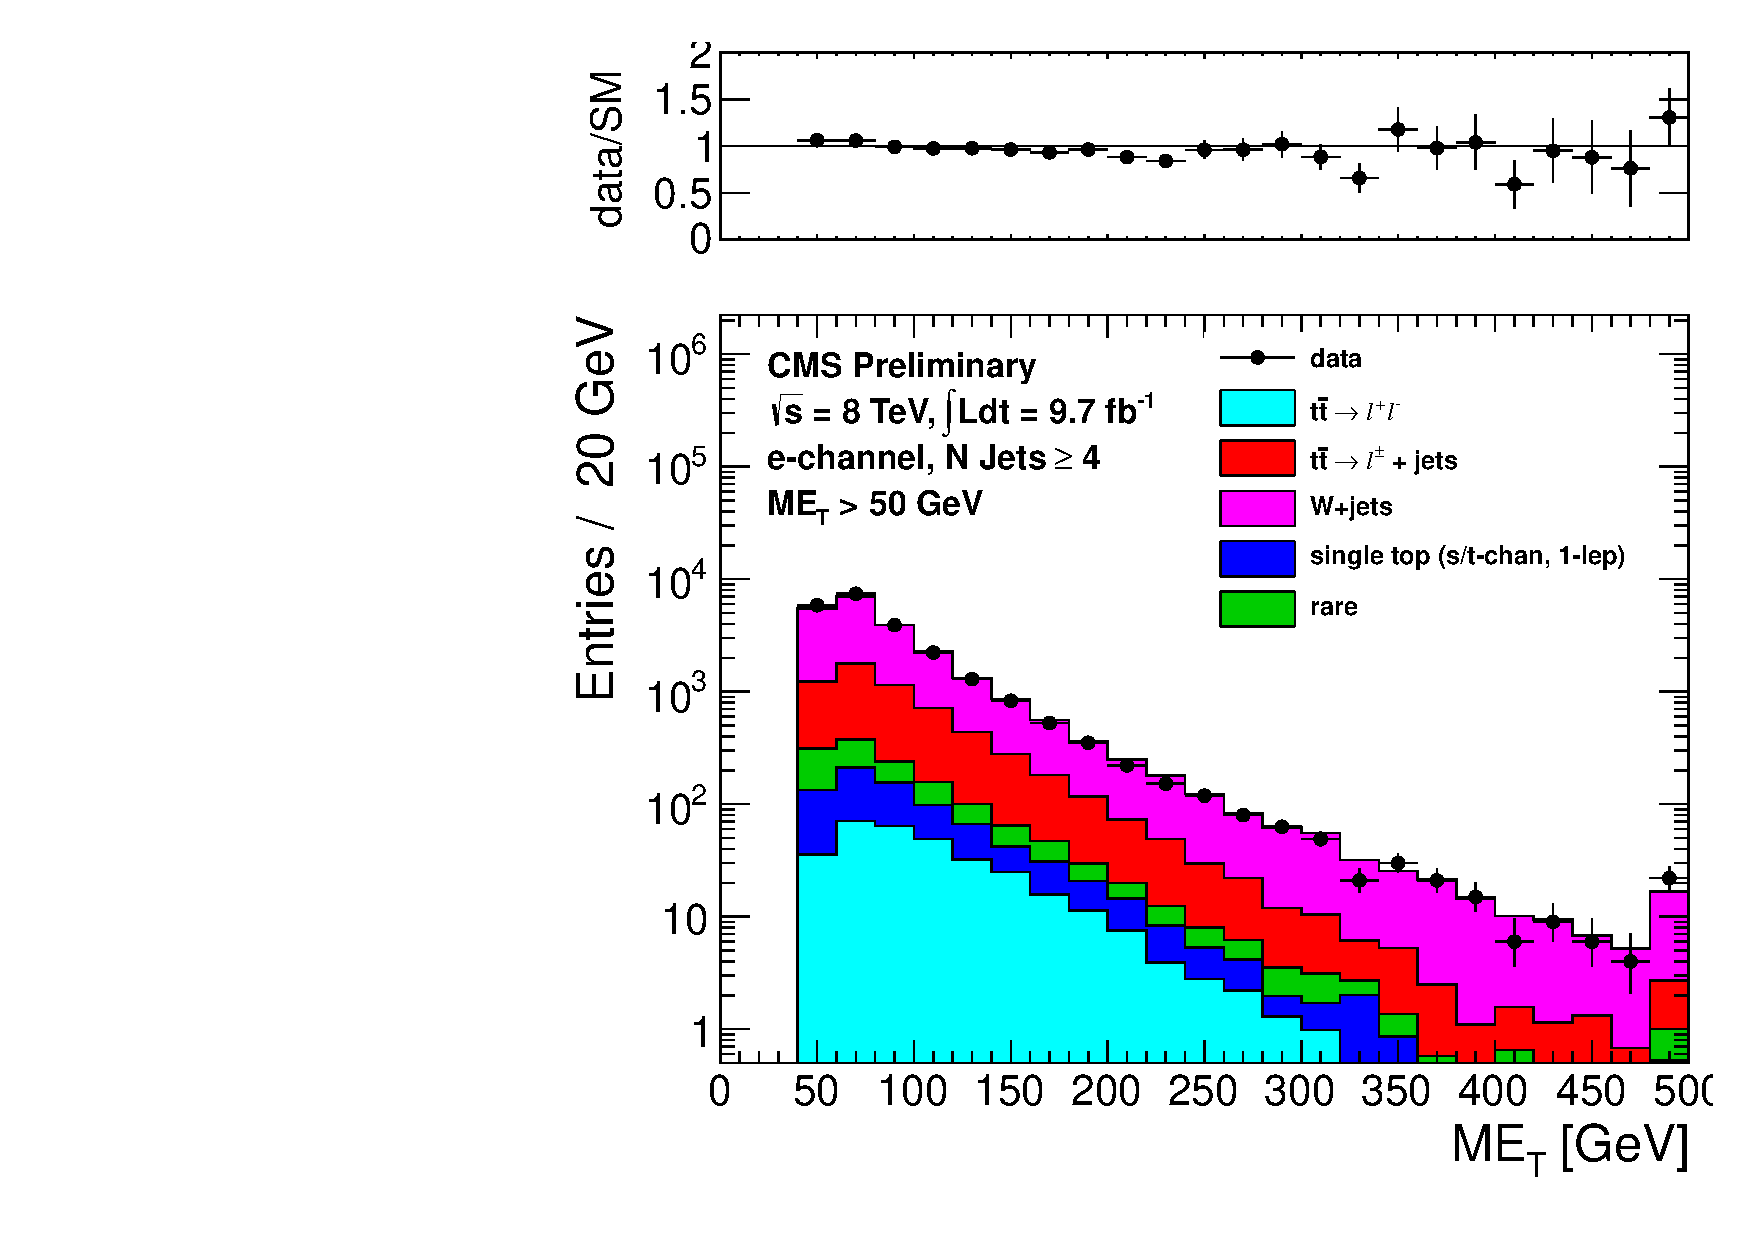
\includegraphics[width=0.5\linewidth]{plots/CR1plots/met_met50_leadele_nj4.pdf}
        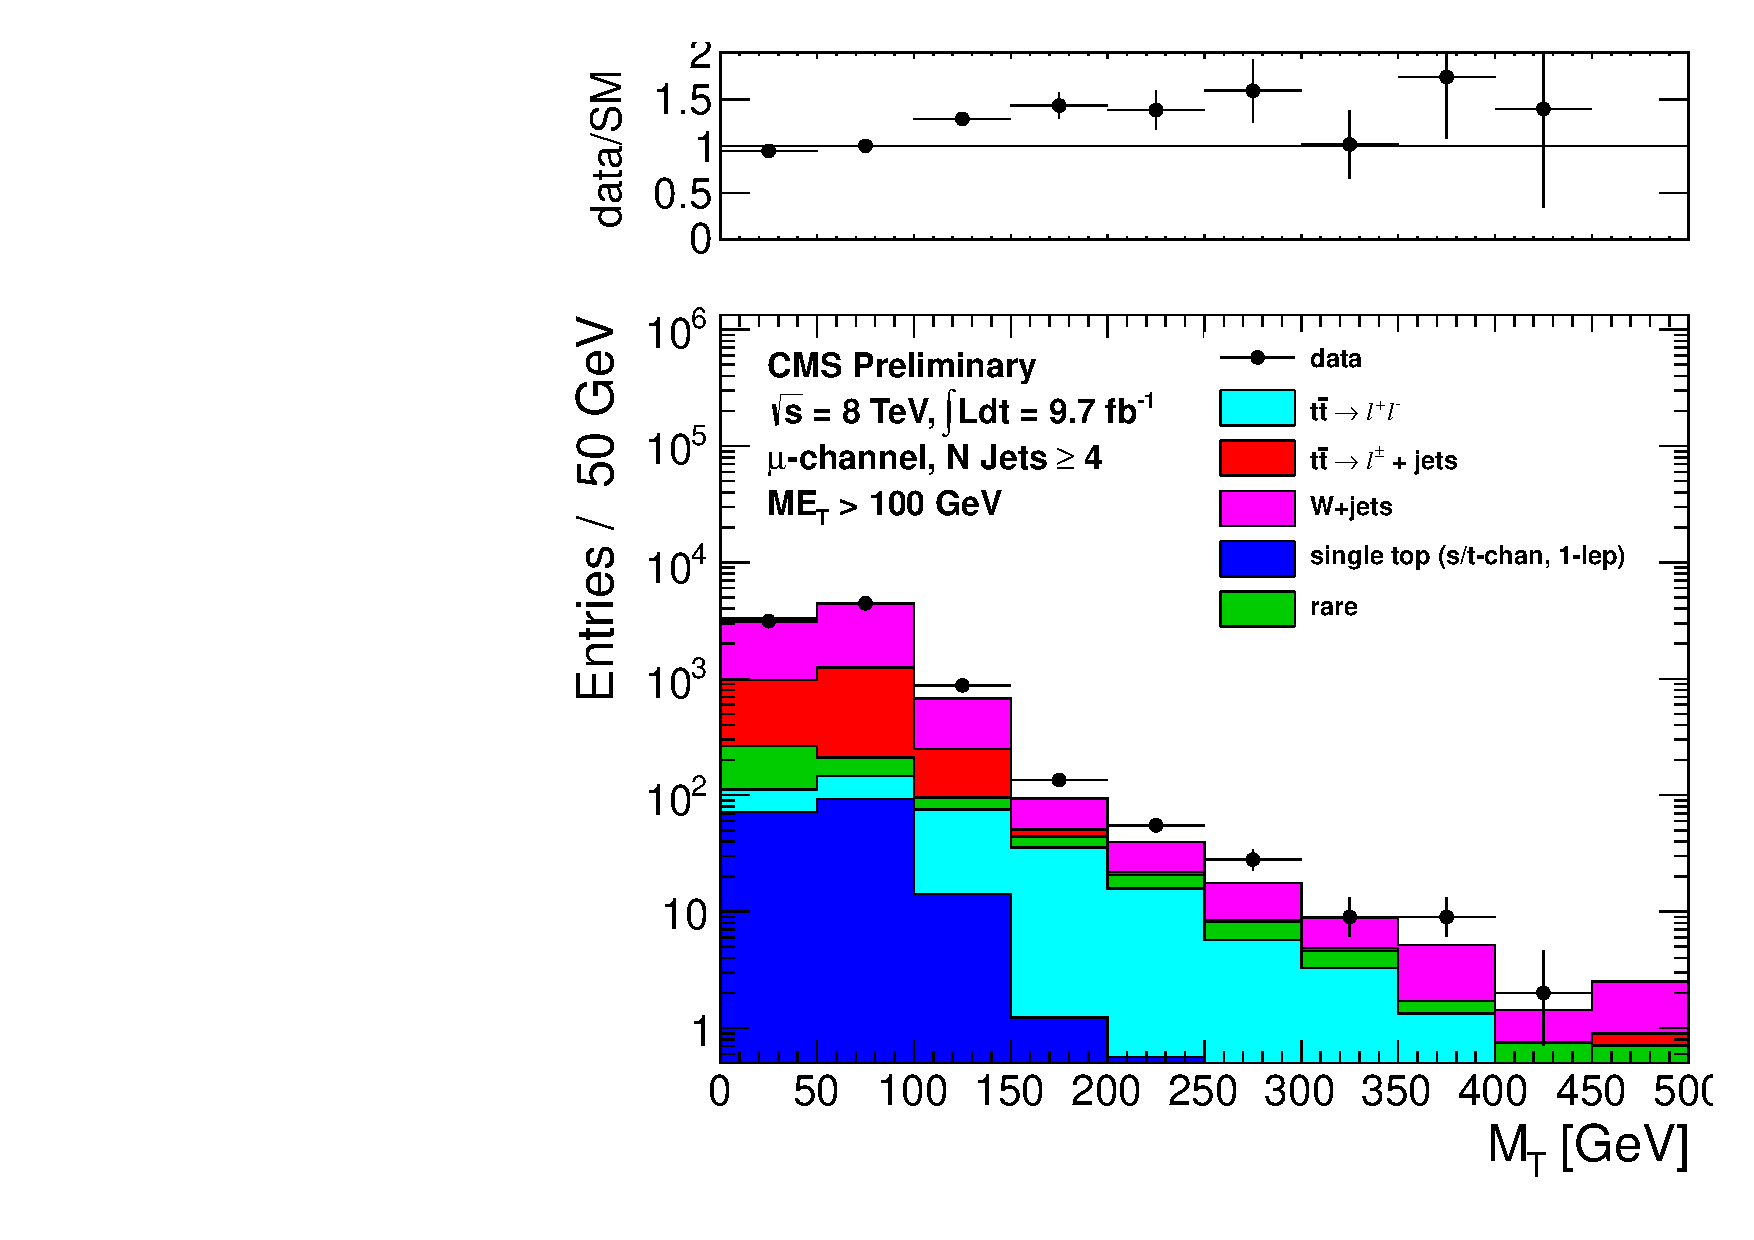
\includegraphics[width=0.5\linewidth]{plots/CR1plots/mt_met100_leadmuo_nj4.pdf}%
        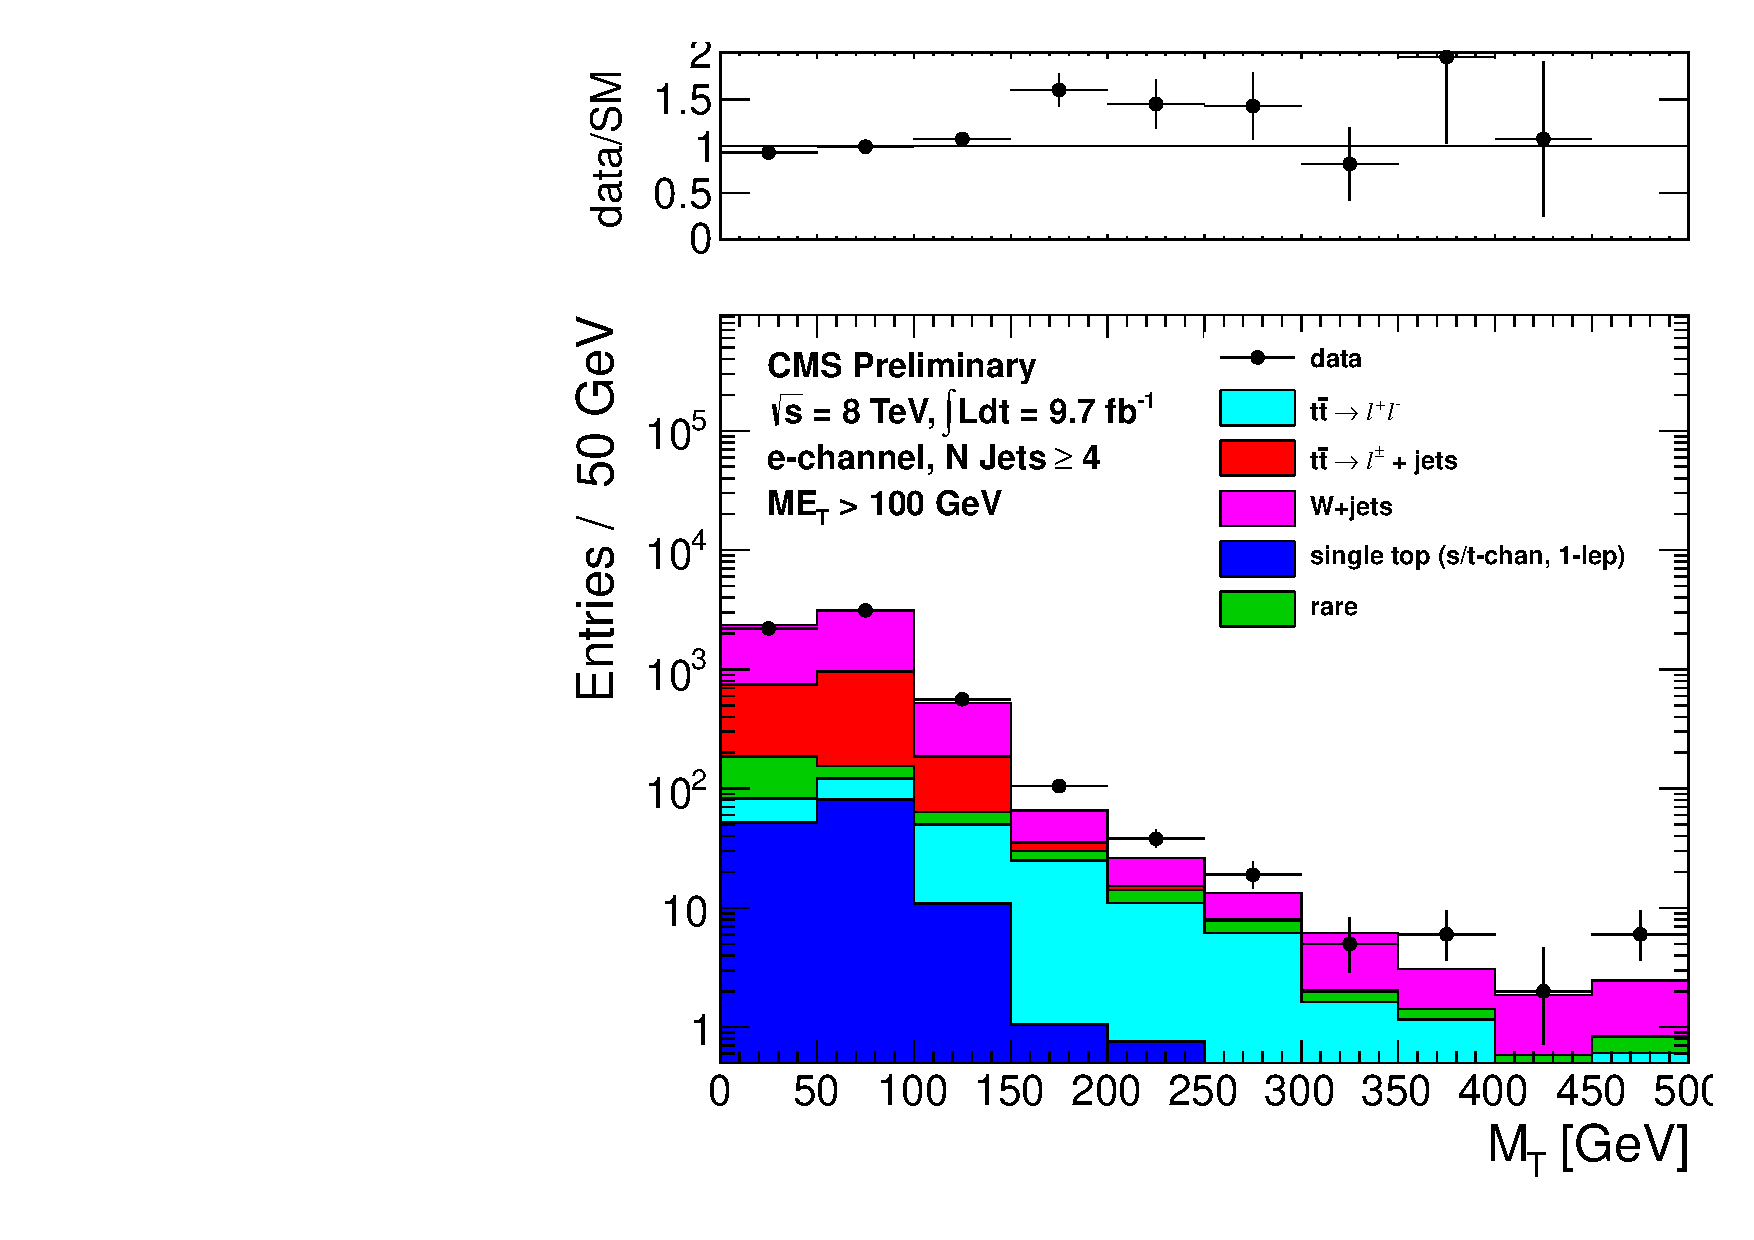
\includegraphics[width=0.5\linewidth]{plots/CR1plots/mt_met100_leadele_nj4.pdf}
    \caption{
      Comparison of the \met\ (top) and \mt\ for $\met>100$ (bottom) distributions in data vs. MC for events
      with a leading muon (left) and leading electron (right)
      satisfying the requirements of CR1. 
\label{fig:cr1met} 
}  
      \end{center}
\end{figure}


\begin{figure}[hbt]
  \begin{center}
        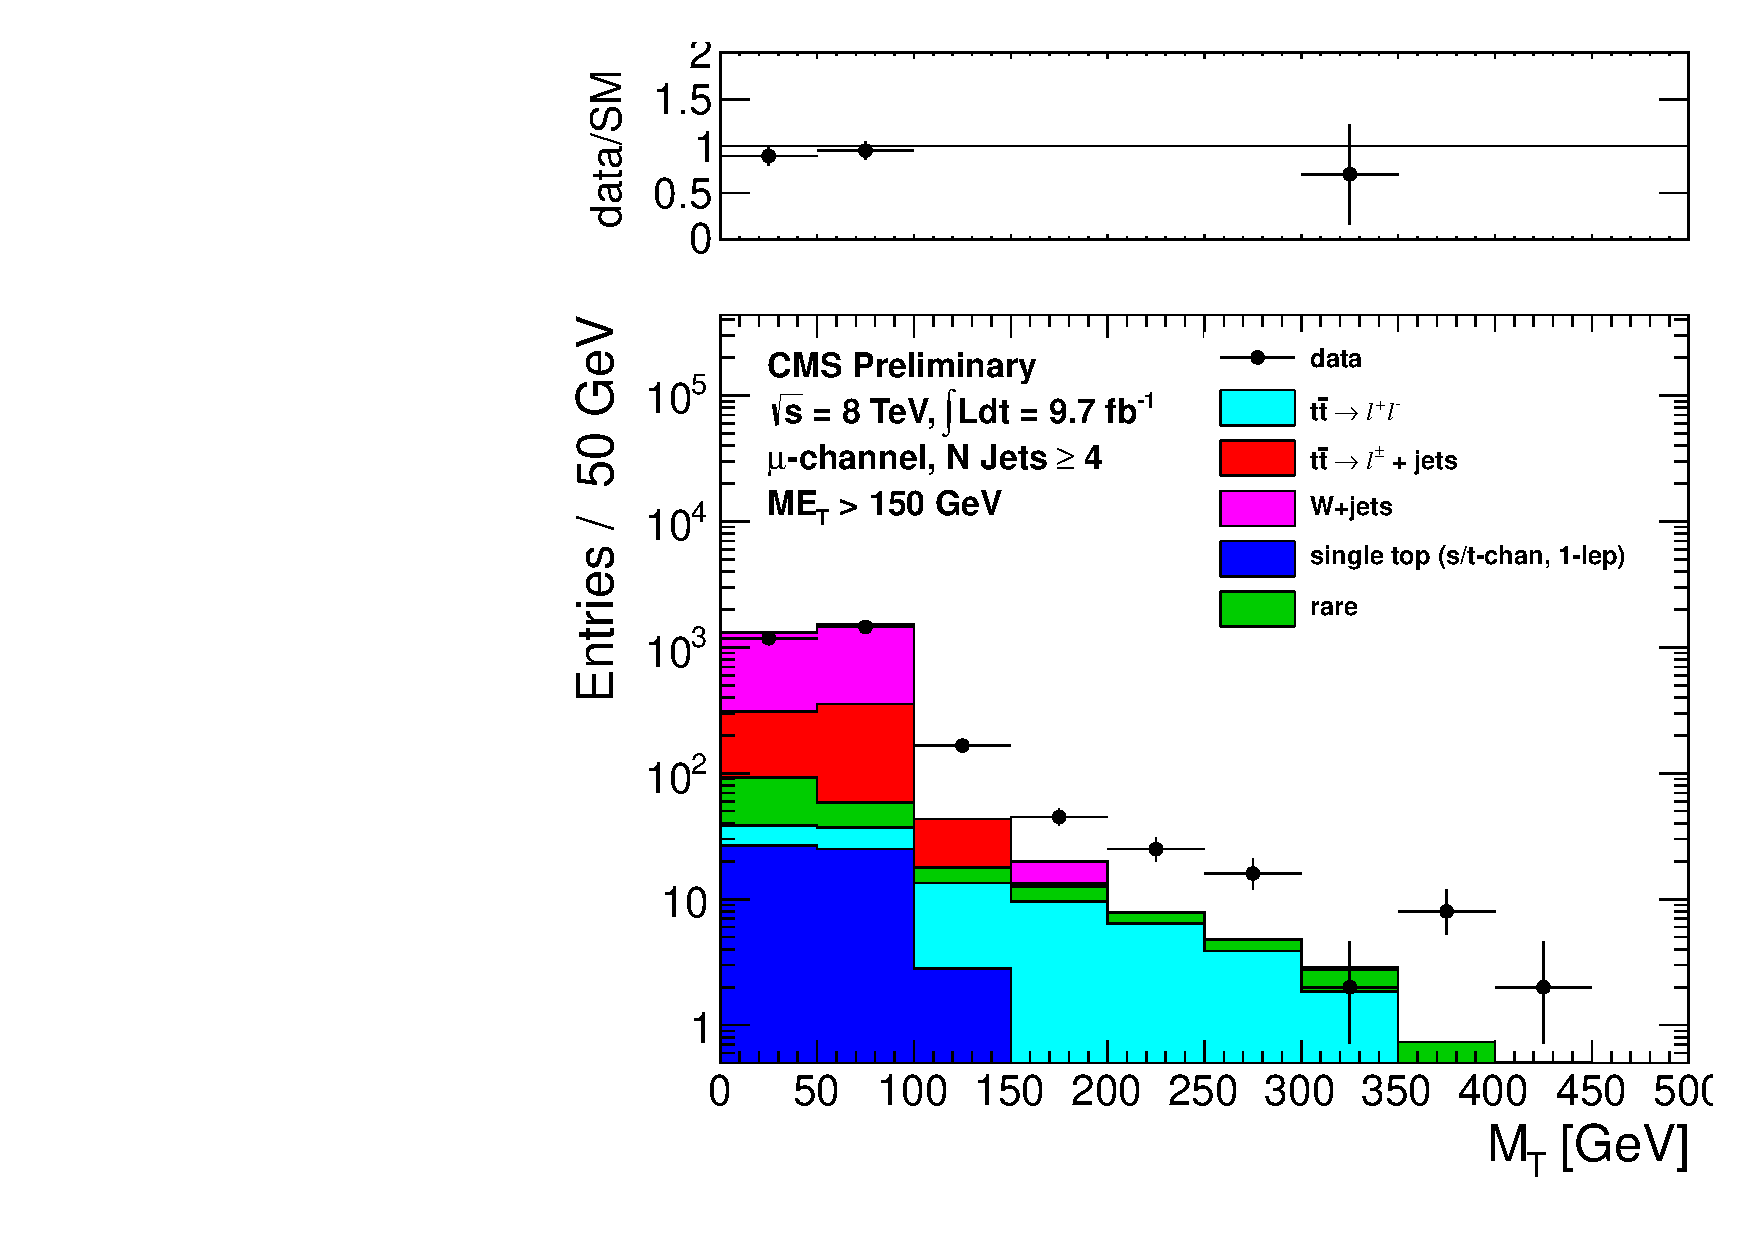
\includegraphics[width=0.5\linewidth]{plots/CR1plots/mt_met150_leadmuo_nj4.pdf}%
        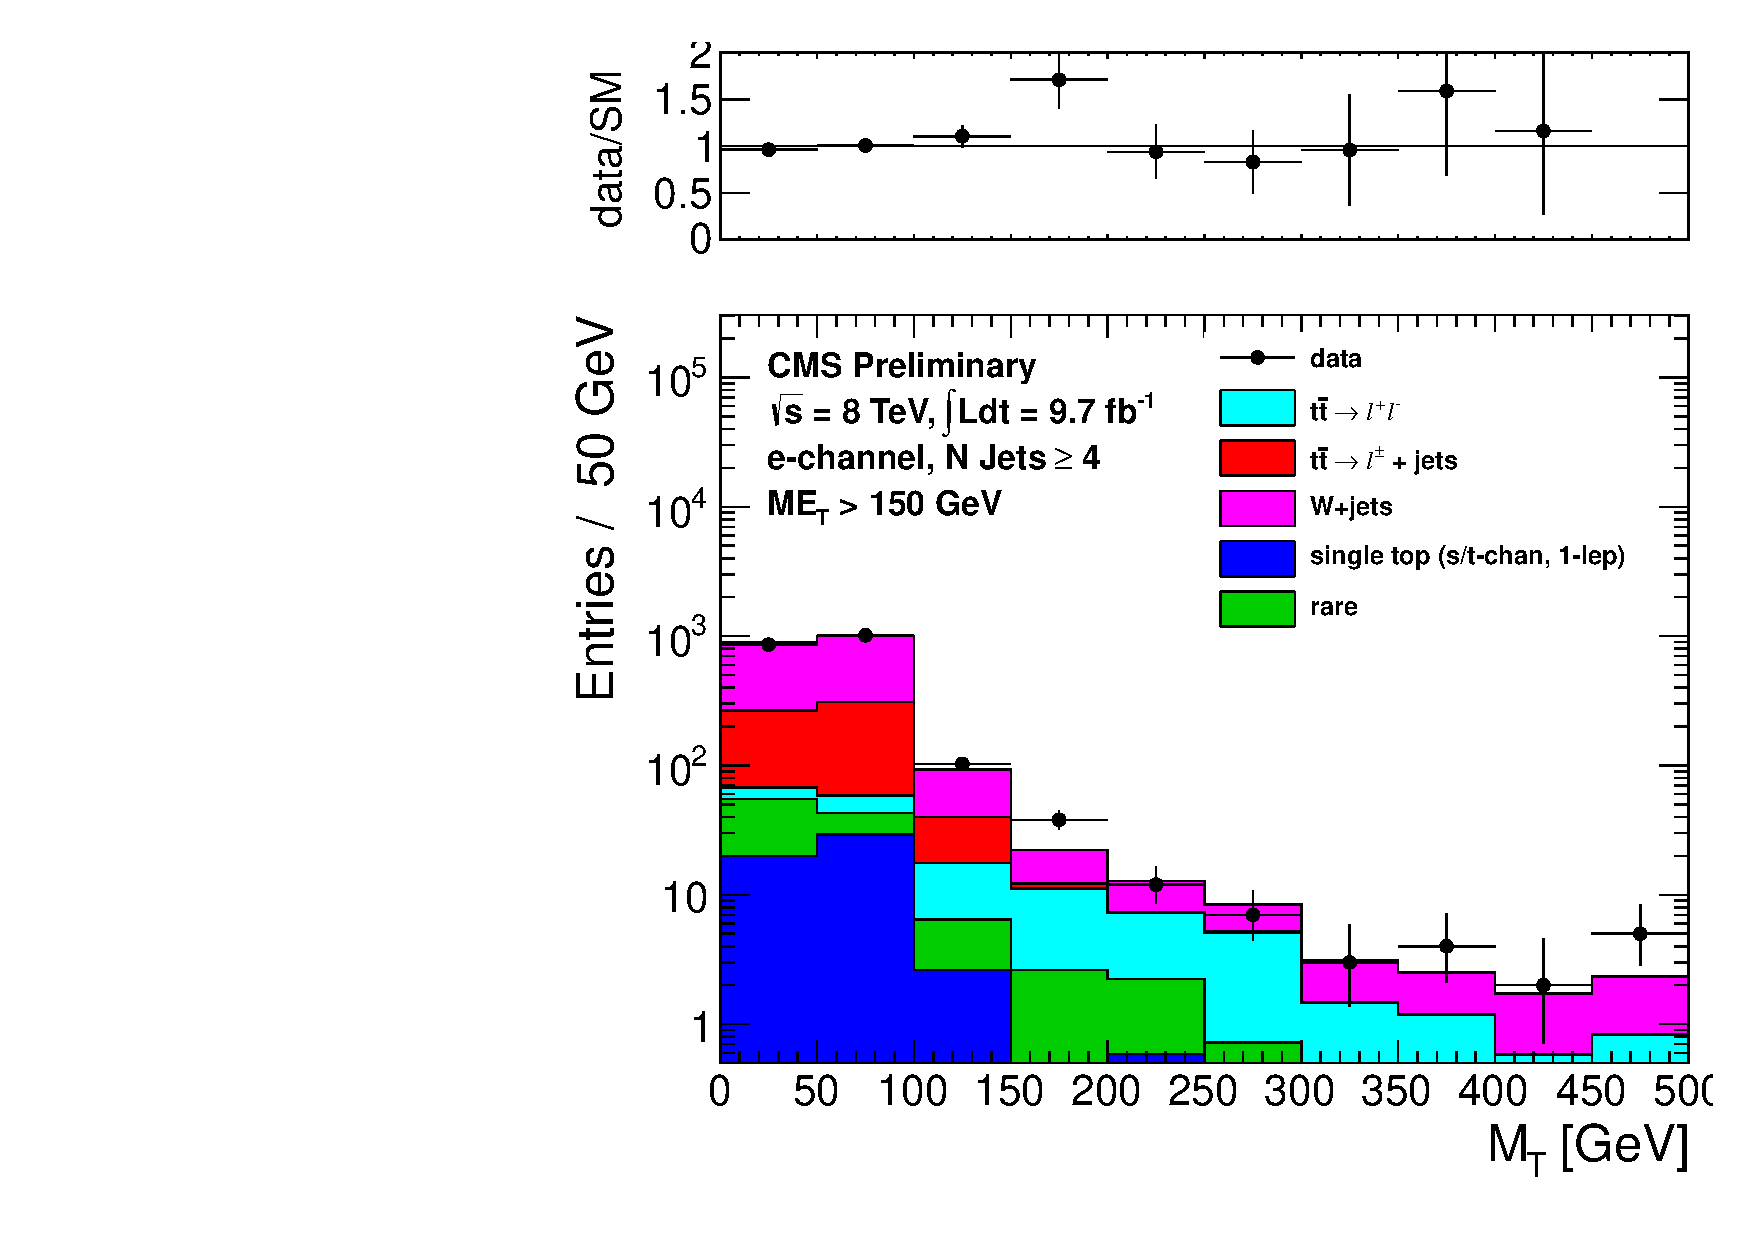
\includegraphics[width=0.5\linewidth]{plots/CR1plots/mt_met150_leadele_nj4.pdf}
        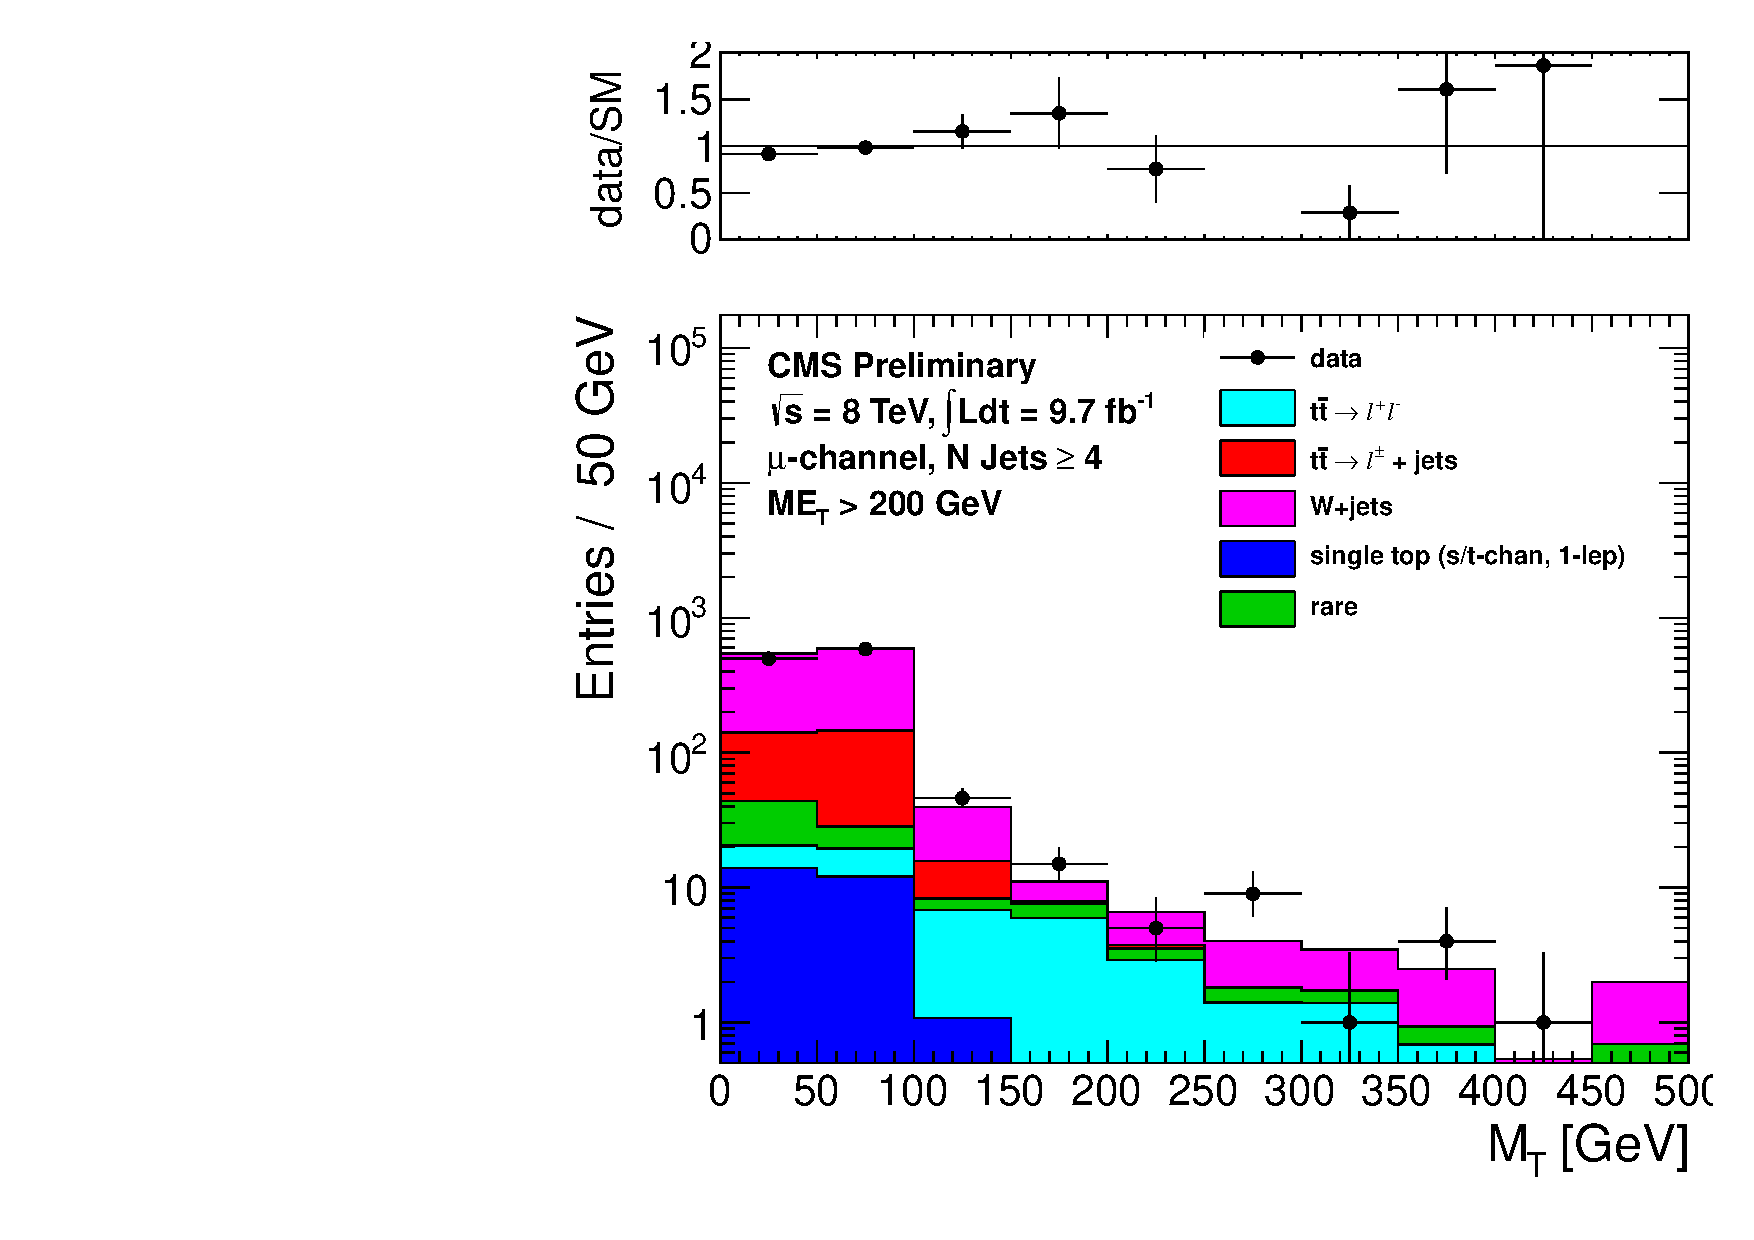
\includegraphics[width=0.5\linewidth]{plots/CR1plots/mt_met200_leadmuo_nj4.pdf}%
        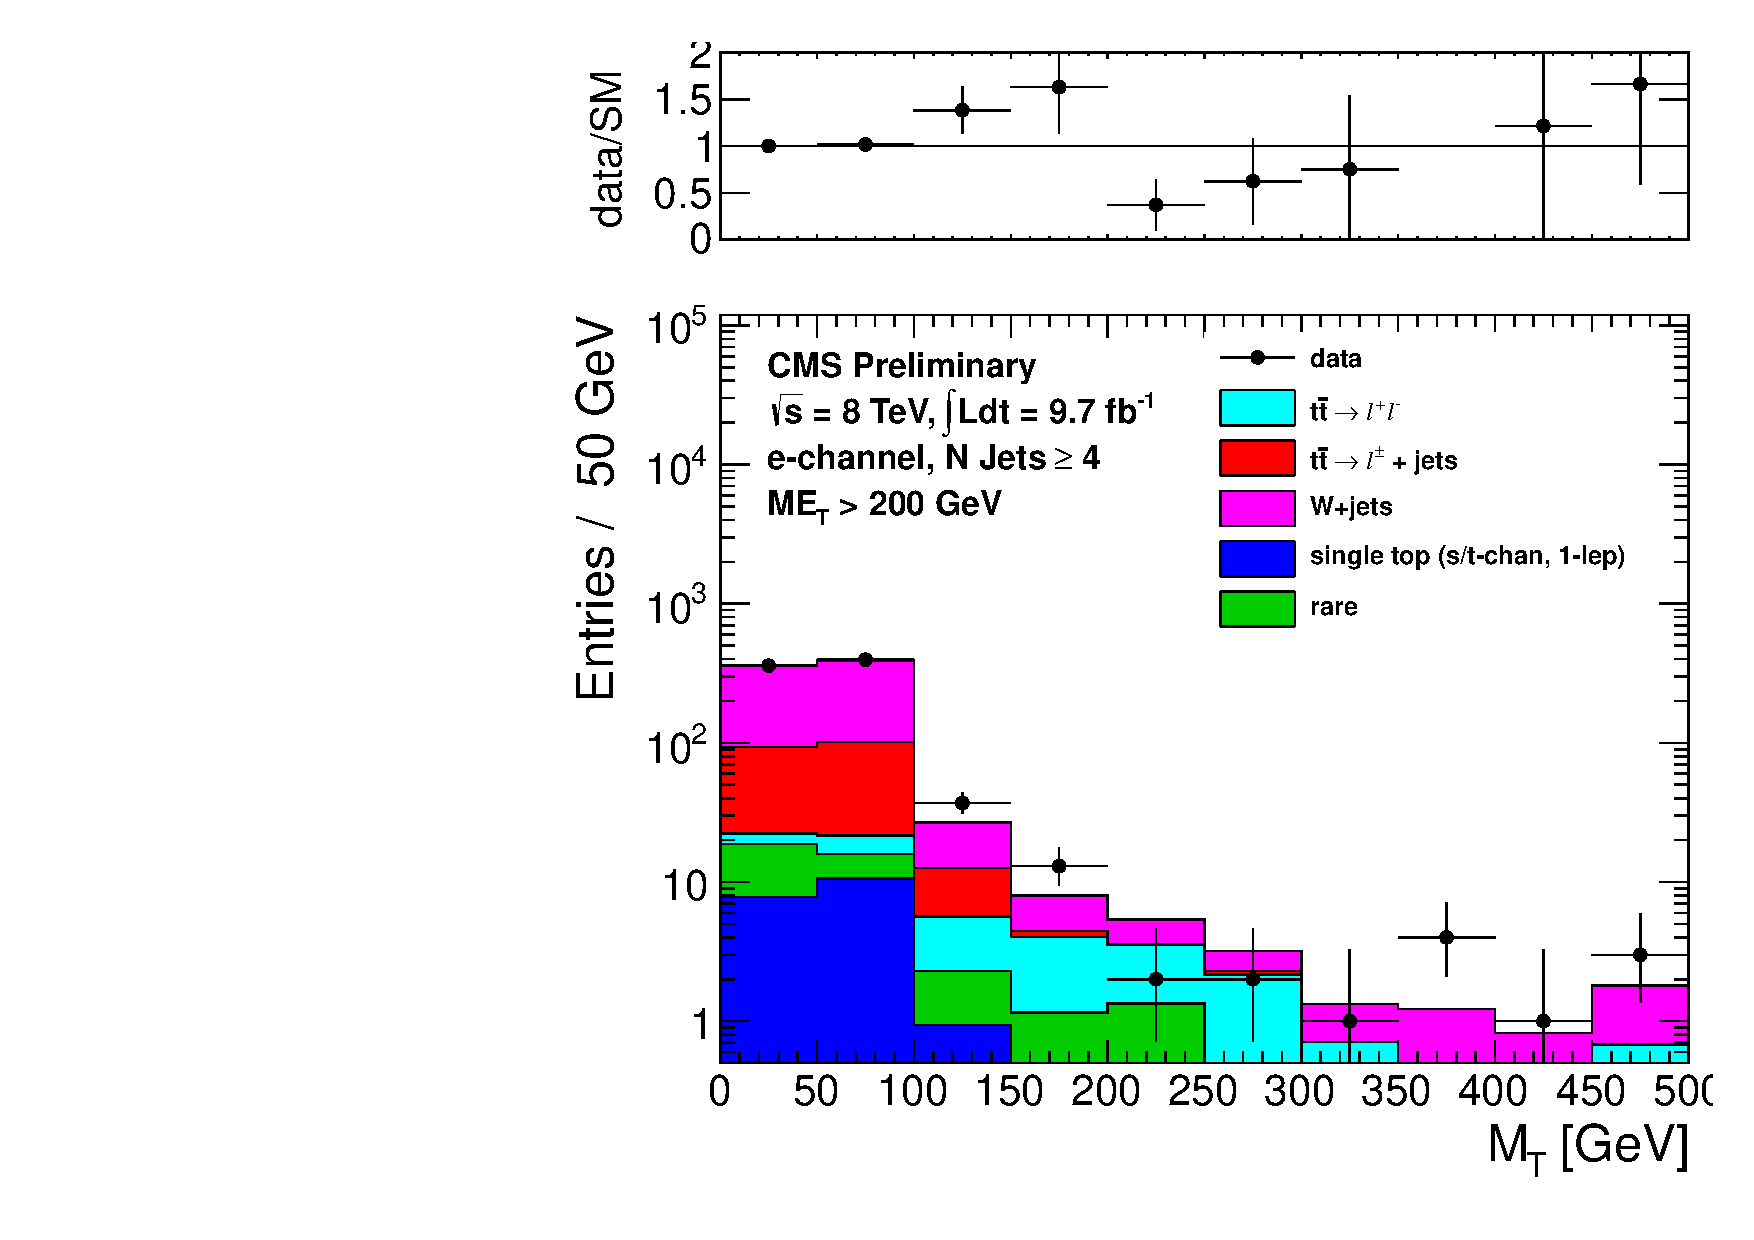
\includegraphics[width=0.5\linewidth]{plots/CR1plots/mt_met200_leadele_nj4.pdf}
        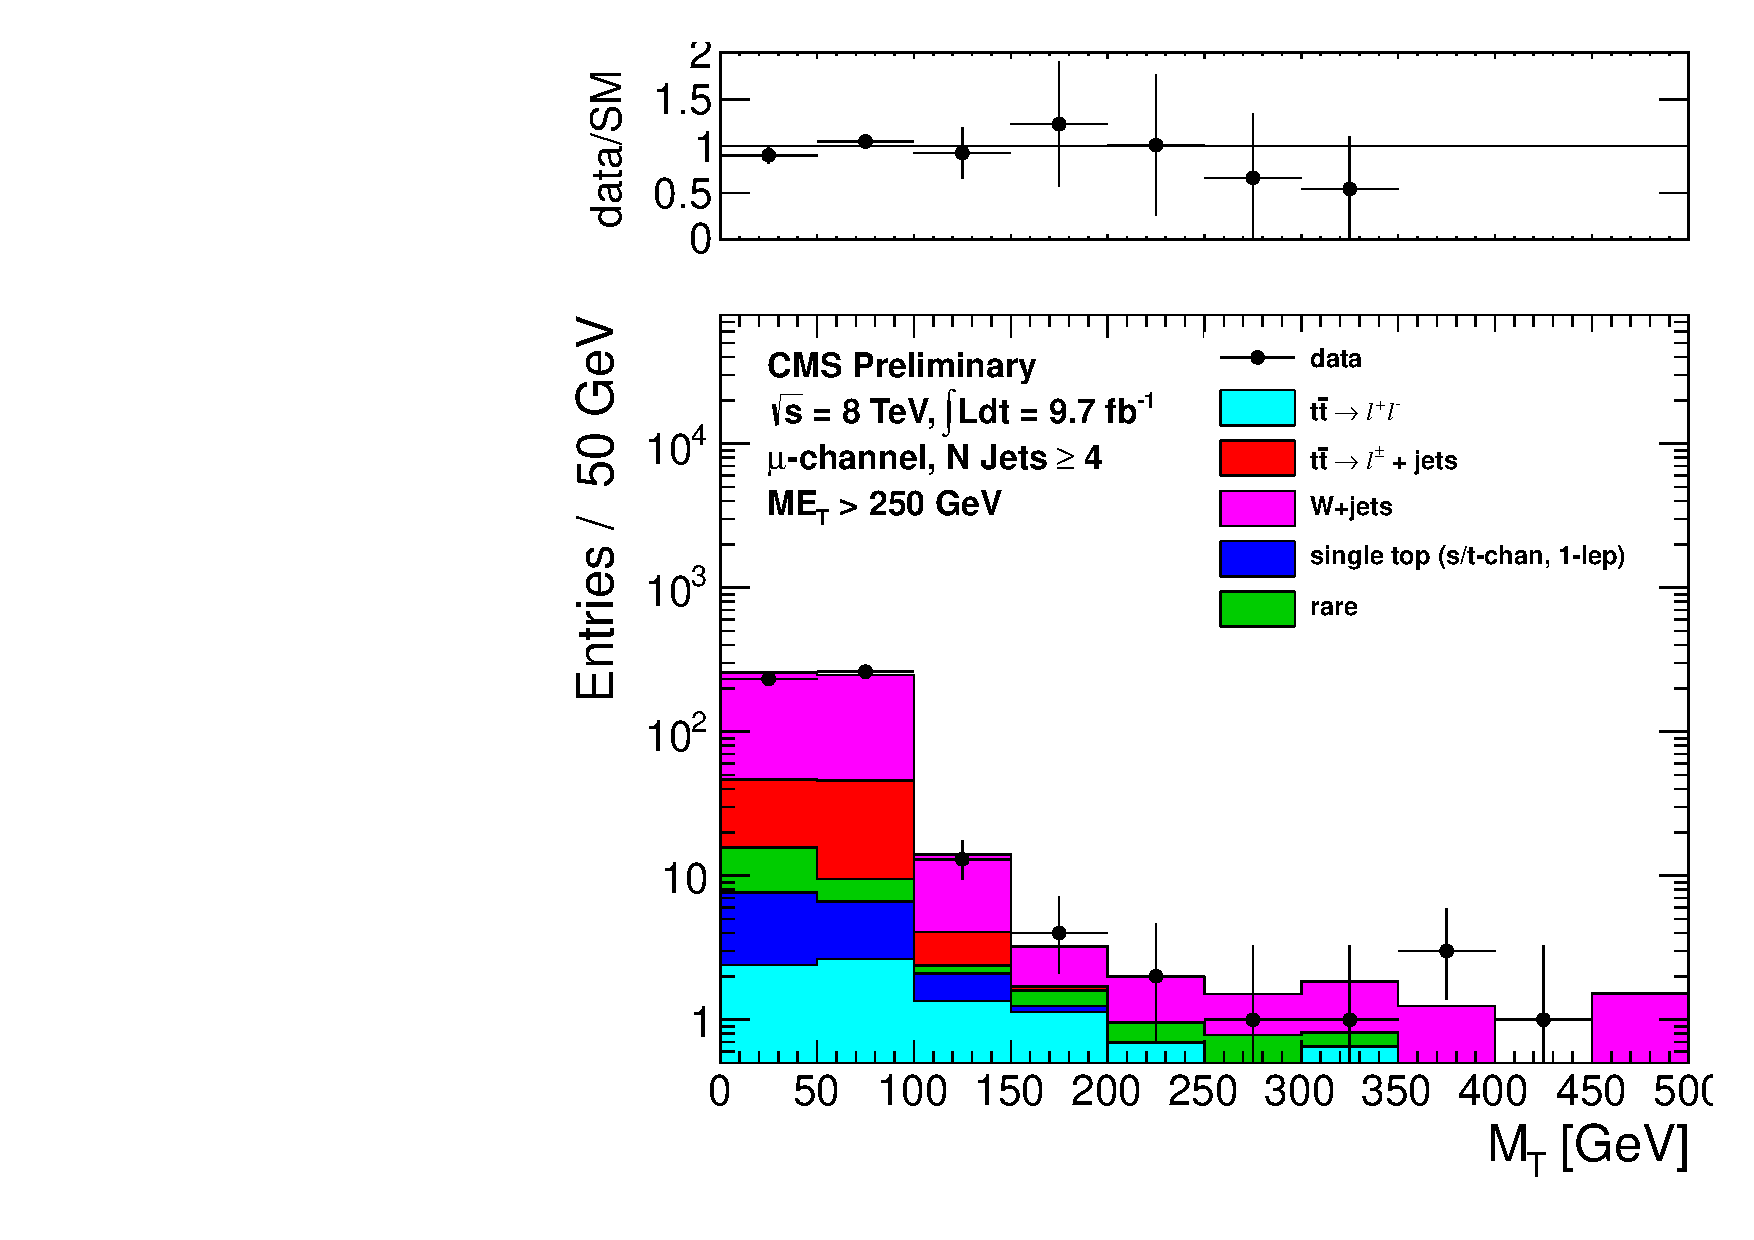
\includegraphics[width=0.5\linewidth]{plots/CR1plots/mt_met250_leadmuo_nj4.pdf}%
        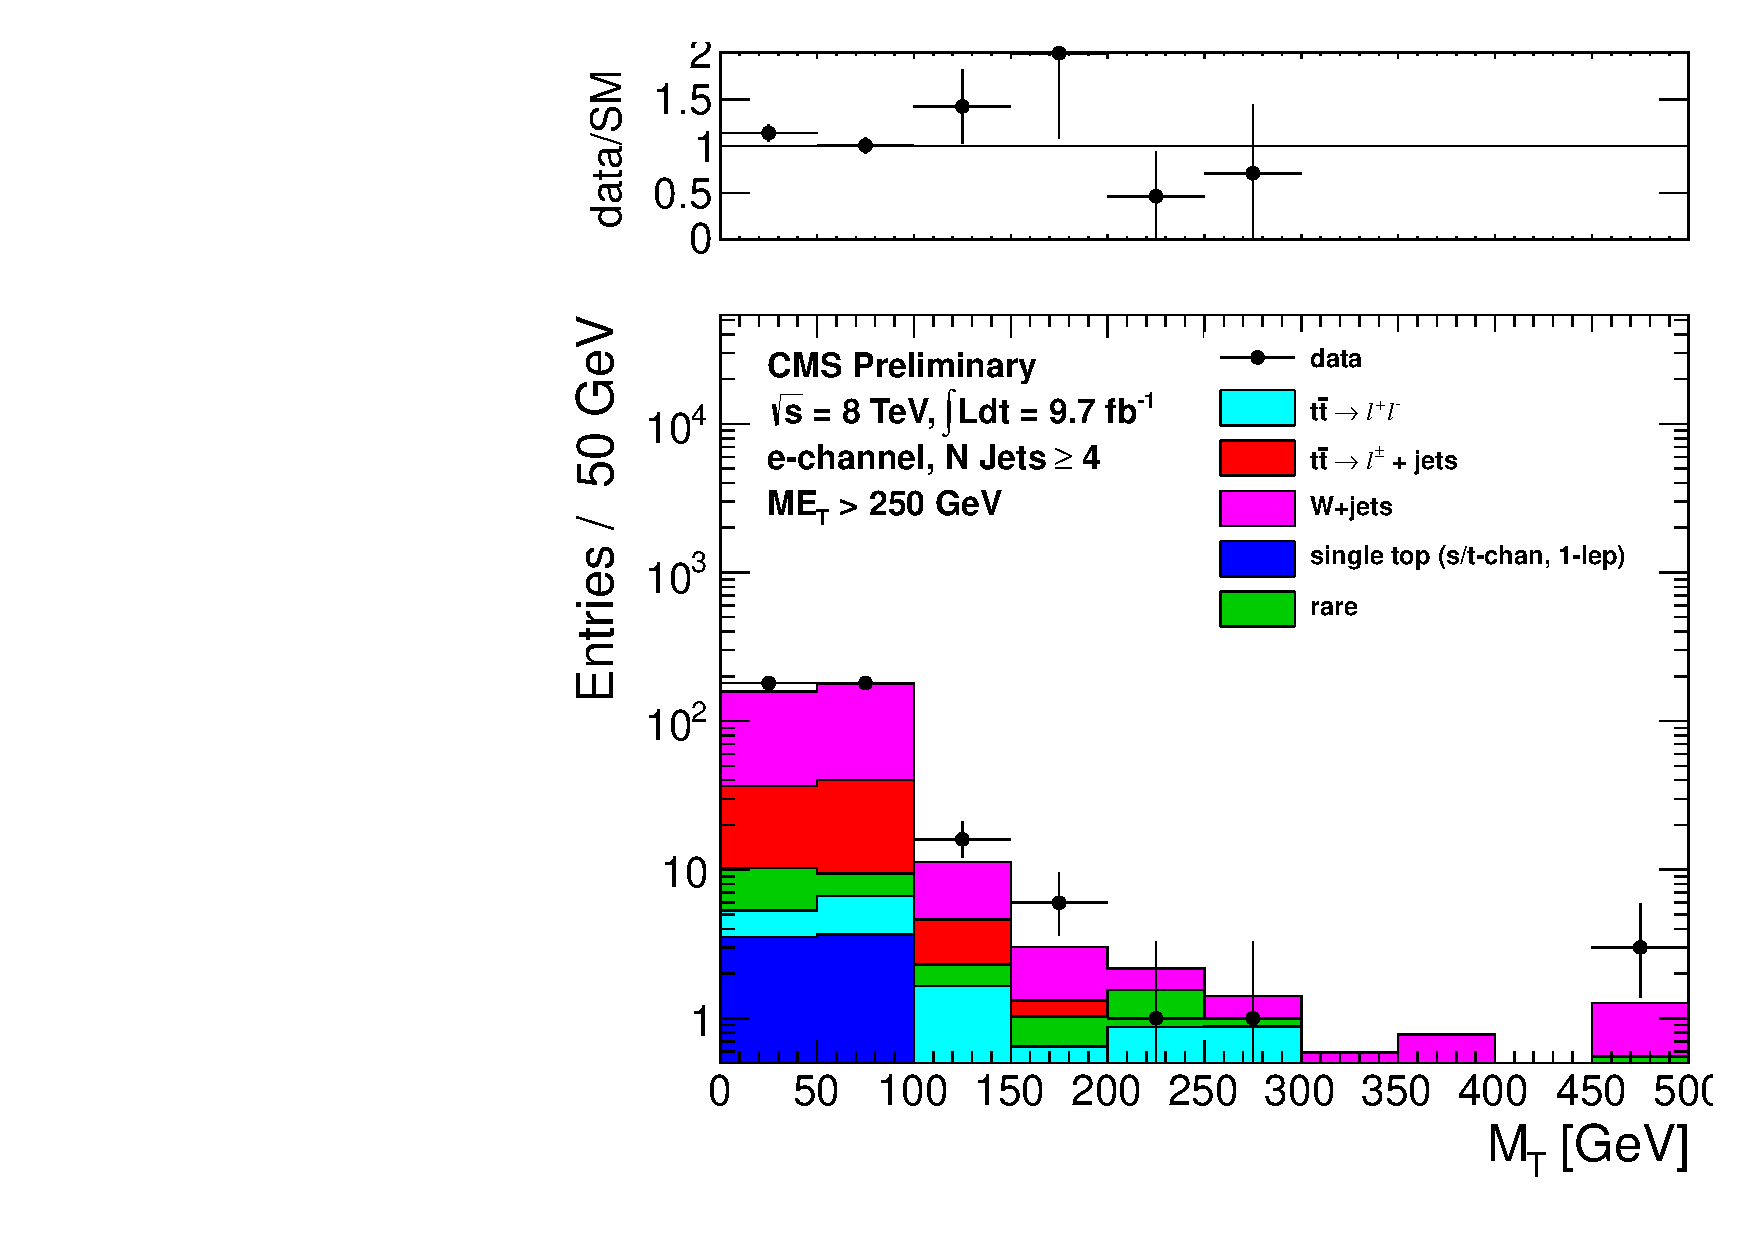
\includegraphics[width=0.5\linewidth]{plots/CR1plots/mt_met250_leadele_nj4.pdf}
    \caption{
      Comparison of the \mt\ distribution in data vs. MC for events
      with a leading muon (left) and leading electron (right)
      satisfying the requirements of CR1. The \met\ requirements used are
      150 GeV (top), 200 GeV (middle) and 250 GeV (bottom).
\label{fig:cr1mtrest} 
}  
      \end{center}
\end{figure}

\clearpage